\section{Diffusion Process: The Heat Kernel}

\subsection{The Heat Equation on a Graph Manifold}
The Laplacian matrix is not only useful for studying static network structures or discrete oscillations, but it is also the fundamental operator for describing \textbf{diffusion processes} on a graph manifold.

The definition of the diffusion process on a network is the direct discrete analogue of the continuous \textbf{Heat Equation}. In continuous physics, the diffusion of heat (or probability density) $p(x,t)$ is governed by the second spatial derivative:
\[
    \dot{p}(x) = -D \frac{d^2}{dx^2}p(x)
\]
which has the classic Gaussian solution over time:
\[
    p(x,t) = C \cdot e^{-\frac{x^2}{2\sigma^2 \cdot t}}
\]

On a discrete graph manifold, the second derivative is replaced by the Laplacian operator \( L \). The differential equation governing the diffusion of a state vector \( \vec{x} \) (which could represent heat, probability, or information at each node) over time becomes:
\[
    \dot{\vec{x}} = -L\vec{x}
\]
The formal mathematical solution to this linear differential equation is given by the matrix exponential:
\[
    \vec{x}(t) = e^{-Lt} \vec{x}(0)
\]
where \( \vec{x}(0) \) is the initial state configuration at time \( t=0 \).
The core of this solution is the matrix \( H \), known as the \textbf{Heat Kernel}:
\[
    H = e^{-Lt}
\]

\textit{References:}
\begin{itemize}
    \item Hancock ICIAR08; Kondor \& Lafferty Proc02 (available on Virtuale).
    \item \textbf{Historical Note:} Ricci flows on manifolds (a generalized diffusion process) are at the absolute basis of Grigori Perelman's demonstration of the Poincaré conjecture [Arxiv21, SciRep19].
\end{itemize}

\subsection{Shortest Paths}
To compute or approximate the Heat Kernel, we rely on the expansion of the exponential function into a power series (Taylor series). For a standard scalar \( x \):
\[
    e^x = 1 + \frac{x}{1!} + \frac{x^2}{2!} + \frac{x^3}{3!} + \dots + \frac{x^n}{n!} + \dots
\]
Which can be written compactly as:
\[
    e^x = 1 + \sum_{n=1}^{\infty} \frac{1}{n!} x^n = \sum_{n=0}^{\infty} \frac{1}{n!} x^n
\]
Applying this definition to our matrix \( -Lt \), we obtain the series expansion for the Heat Kernel:
\[
    e^{-Lt} = \sum_{n=0}^{\infty} \frac{1}{n!} (-Lt)^n
\]
One can equate this to \( e^{-t}(I - L + \frac{L^2}{2} + \dots) \). Strictly speaking, the standard Taylor expansion evaluates to \( I - Lt + \frac{t^2 L^2}{2} - \dots \). The expression refers to a specific normalization or evaluation at \( t=1 \), but the fundamental concept remains: the Heat Kernel incorporates information from all powers of the Laplacian. Because \( L^n \) counts paths of length \( n \), the Heat Kernel inherently aggregates \textbf{shortest path} and global connectivity information across the entire network.

\subsection{Node Coordinates}

We can use the Heat Kernel to represent nodes in an \( N \)-dimensional space. Because \( L \) is symmetric, \( H \) is also symmetric and positive-definite. We can decompose \( H \) into the product of two identical matrices (Young-Householder decomposition):
\[
    e^{-Lt} = H = \Phi \Lambda_H \Phi^T = Y Y^T
\]
It can be written as \( \Phi \Lambda \Phi^T \), where \( \Lambda \) here specifically represents the diagonal matrix of the exponentiated eigenvalues \( e^{-t\lambda_i} \).

We can define the embedding matrix \( Y \), where each column represents a node:
\[
    Y = (y_1 | y_2 | \dots | y_{|V|}) = \exp\left[-\frac{1}{2}t\Lambda\right] \Phi^T
\]
This Heat Kernel representation strongly depends on the \textbf{evolution time \( t \)}. Every node is represented as a vector of \( Y \) components, which are essentially the eigenvectors \( \Phi_i \) rescaled by the exponential of their eigenvalues.

From this decomposition:
\begin{enumerate}
    \item Nodes can be \textbf{embedded} into a reduced \( k \)-dimensional space by selecting only the first \( k \) eigenvectors.
    \item The Euclidean squared \textbf{distances} \( d_E^2(u,v) \) between nodes \( u \) and \( v \) in this embedded space can be calculated exactly:
          \[
              d_E^2(u, v) = (y_u - y_v)^T (y_u - y_v) = \sum_{i=1}^{|V|} \exp[-\lambda_i t] (\phi_i(u) - \phi_i(v))^2
          \]
          Node coordinates can then be remapped using Multi-Dimensional Scaling (MDS) on this calculated distance matrix \( D \).
\end{enumerate}

\subsection{Spectral Decomposition and the Role of Time}

The Heat Kernel can be fully decomposed onto the eigenvector basis \( \Phi \) of \( L \), creating an \( N \)-dimensional embedding:
\[
    Y = (y_1 | y_2 | \dots | y_{|V|}) = \exp\left[-\frac{1}{2}t\Lambda\right] \Phi^T
\]
The structure of this embedding changes drastically depending on the parameter \( t \):
\begin{itemize}
    \item \textbf{For small \( t \):} The expansion is dominated by the linear term:
          \[
              H_t \approx I - Lt
          \]
          At this scale, diffusion has barely started, so the kernel strictly depends on the immediate, local \textbf{network topology} (who is directly connected to whom).

    \item \textbf{For large \( t \):} The higher-order terms decay, and the long-term behavior is dominated by the smallest non-zero eigenvalue:
          \[
              H_t \approx \Phi \exp(-\lambda_2 t) \Phi^T
          \]
          At this macroscopic scale, the diffusion depends almost entirely on the \textbf{Fiedler vector} and the global bottlenecks of the network.
\end{itemize}
By modulating \( t \), we can obtain different representations of the same network. Thus, \textbf{time} acts as a \textbf{parameter} that can be optimized in relation to a specific cost function (e.g., maximizing classification/regression performance, or optimizing modularity indexes for community detection).

\subsubsection{The Heat Kernel as a Low-Frequency Pass Filter}
Because the embedding relies on the exponential decay term \( \exp[-\lambda_i t] \), the eigenvalues dictate the decay rate of their corresponding eigenvectors.

For an increasing time \( t \), the eigenvectors related to the \textbf{highest eigenvalues} (the "higher frequencies" of the graph, representing noisy, local, highly fluctuating structural details) \textbf{disappear first}.
\begin{itemize}
    \item These are \textbf{fastly decaying transient modes}.
    \item \textbf{High frequency modes decay faster.}
\end{itemize}

Consequently, Heat Kernel diffusion acts mathematically as a \textbf{low-frequency pass filter}. It smooths out local irregularities and highlights the macro-structures (communities, major pathways) of the graph.
\textit{(Reference: image smoothing Zhang Hancock PatRec08).}

\subsection{Heat Kernel Evolution and Phase Transitions}

During the diffusion process, network dynamics do not always evolve smoothly and uniformly towards the stationary state. Depending on the topology, the diffusion can remain "stuck" in \textbf{transient states} for extended periods during its evolution. For instance, in a network with a strong community structure, the diffusion quickly equilibrates within local, densely connected clusters, but it takes a significantly longer time to traverse the sparse bottlenecks between different clusters.

This step-wise evolution mirrors phenomena observed in other complex physical systems. A notable example is the cascades of \textbf{phase transitions} seen during the evolution of Potts multi-spin models in statistical mechanics. This concept is directly exploited in algorithms like \textit{superparamagnetic clustering} [E. Domany PRL96], where different communities "melt" and merge at different simulated temperatures (or times).

\subsection{General Applications of the Heat Kernel}
The heat kernel provides a highly robust framework for evaluating similarities between nodes. Nodes (which could represent anything from social actors to image pixels) can be quantitatively compared through their \( K \)-dimensional \textbf{embedding representation} \( Y_k \) derived from the spectral decomposition of the heat kernel.

By evaluating the Euclidean distances in this embedded space, the method can be effectively used for:
\begin{itemize}
    \item \textbf{Node clustering:} Grouping nodes into communities based on how easily "heat" flows between them.
    \item Identifying \textbf{similar nodes} or isolating disconnected \textbf{outlier nodes}.
\end{itemize}

When setting up this framework, the researcher has several options and parameters to define:
\begin{enumerate}
    \item \textbf{Choice of the Operator:} Deciding whether to use the "original" oscillatory Laplacian (\( L \)) or the "normalized" Laplacian (\( L^{(3)} \)).
    \item \textbf{Choice of Network Weights:} Defining how edge weights are calculated (e.g., using the difference in pixel intensity in an image, or physical distances).
    \item \textbf{Neighborhood Definition:} Choosing the number of neighbours in the original dataset to calculate proximity. This can be done by connecting a fixed number of nearest neighbors (\( k \)-NN graph) or by connecting all nodes within a fixed "radius" (\( \epsilon \)-neighborhood graph).
\end{enumerate}

\subsubsection{Application to Images: Smoothing and Noise Removal}
A prominent, practical application of the heat kernel is in computer vision for \textbf{image smoothing}. The goal here is to achieve noise removal while simultaneously keeping fine details and edge contrasts intact (\textit{Reference: Zhang Hancock Pat Rec 08}).

To apply network theory to an image, we must map the pixel grid to a graph. An \( N \times M \) pixel image is flattened into a single 1D pixel vector of size \( NM \). Consequently, the underlying network representation connects these pixels, resulting in an \( (NM) \times (NM) \) Laplacian matrix \( \mathcal{L} \).

The diffusion process is modeled by the standard initial value problem for the heat equation, applied to the time-dependent pixel vector \( \vec{u}_t \):
\[
    \begin{cases}
        \frac{\partial \vec{u}_t}{\partial t} = -\mathcal{L} \vec{u}_t \\
        \vec{u}_0 = \vec{\mathcal{I}}
    \end{cases}
\]
Here, the initial condition \( \vec{u}_0 \) is simply the vector of the original pixel intensities \( \vec{\mathcal{I}} \).

The smoothed intensity of any specific pixel \( j \) at time \( t \) is obtained by applying the Heat Kernel \( H_t \) to the initial conditions. It is calculated as the sum of the initial intensities of all vertices \( i \) in the volume \( |V| \), weighted by the heat kernel's transition value between \( i \) and \( j \):
\[
    \vec{u}_t(j) = \sum_{i=1}^{|V|} \vec{\mathcal{I}}(i) \times H_t(i,j)
\]
As \( t \) acts as a low-pass filter parameter, increasing \( t \) progressively smooths the image, filtering out high-frequency noise while structural boundaries (which act as bottlenecks in the pixel graph) temporarily resist the diffusion, preserving the edges.

\subsubsection{Network Construction from Images: Pixel Distance and Radius}
To apply the Laplacian and Heat Kernel formalism to images, we must first construct the network representing the image. A standard approach is to define a weighted Laplacian \( L = D - W \), where the weights are based on the \textbf{pixel intensity differences} \( d_{ij} \) within a fixed spatial distance \( r \) on the image.

The weight \( w(i,j) \) between pixel \( i \) and pixel \( j \) is typically defined using a Gaussian kernel, but constrained by a physical radius:
\[
    w(i,j) =
    \begin{cases}
        \exp\left(-\frac{d^2(i,j)}{\kappa^2}\right) & \text{if } ||X(i) - X(j)||_2 \leqslant r \\
        0                                           & \text{otherwise}
    \end{cases}
\]
Here, \( d(i,j) \) represents the difference in color or intensity between the pixels, while \( ||X(i) - X(j)||_2 \) represents the Euclidean spatial distance between their coordinates on the image grid.

When building this network, there are several crucial \textbf{scaling parameters} to choose:
\begin{itemize}
    \item \textbf{Neighborhood radius \( r \):} The maximum spatial distance between pixel positions to consider them connected.
    \item \textbf{Discrete number of neighbors:} Alternatively, instead of a fixed radius, one can connect each pixel to its \( k \)-Nearest Neighbors (KNN).
    \item \textbf{Scaling factor \( \kappa \):} This parameter controls the width of the Gaussian kernel, determining how strictly intensity differences penalize the connection weight.
\end{itemize}

\textit{Note on data normalization:} Pixel intensity differences can (and usually should) be rescaled to the range [0, 1]. This ensures that the weight calculation is independent of the overall image brightness or absolute intensity scale.

\subsection{Time Evolution and Different Representations}
The greatest strength of the Heat Kernel is that it provides a \textbf{combination of all eigenvectors at once}, seamlessly governed by the \textbf{time parameter \( t \)}.

A different value of \( t \) generates a completely different weighting of the eigenvectors. Modulating this parameter allows us to highlight different topological and structural properties of the manifold induced by the network. As previously established:
\begin{itemize}
    \item For \textbf{large \( t \)}, high-frequency modes disappear completely, as they represent faster transient states that quickly decay to zero.
\end{itemize}

This time-dependent filtering provides \textbf{different representations} of the initial data transformed into a network. For example, if we take a 2D figure or a 3D object, we can transform it into a network of connected points using a Delaunay triangulation. By varying \( t \) in the resulting Heat Kernel, we can analyze the object at multiple scales of resolution.

\textbf{Key Applications:} This multi-scale representation is heavily used in image recognition and node clustering. By finding the optimal embedding of objects or images, we can map an image recognition problem directly into a network similarity measure (e.g., evaluating how close two images are by calculating their \textbf{spectral distance} in the embedded space).

\subsection{Notes: Filtering and Matrix Simplification}
To summarize the filtering mechanism, the Heat Kernel "naturally" weights the combination of eigenvectors based strictly on the exponential decay of their corresponding eigenvalues. By doing so, it "naturally" produces a lower-and-lower pass filter (a smoothing effect) as time progresses.

However, we are not strictly bound to this natural decay. \textbf{Other eigenvector combinations can be sought} based on the specific information we want to keep. In advanced applications, we might want to manually craft an optimal combination of high- and low-frequency features of the network, rather than just keeping the low frequencies.

Furthermore, we can use the spectral theorem to construct a \textbf{simplified version} of the original Laplacian matrix. This is done by taking a linear combination of the \textbf{matrix projectors} related only to a specific subset of the eigenvectors.

Using Dirac (bra-ket) notation, the reconstructed or simplified matrix \( L' \) can be written as:
\[
    L' = \sum_{\lambda} | \vec{v}_i^{(\lambda)} \rangle \langle \vec{v}_j^{(\lambda)} |
\]
\begin{remark}
    The term \( | \vec{v}^{(\lambda)} \rangle \langle \vec{v}^{(\lambda)} | \) represents the outer product of the eigenvector associated with eigenvalue \( \lambda \), which acts as a projection matrix onto that 1D subspace. By summing only over a chosen subset of eigenvalues \( \lambda \), we obtain a lower-rank approximation of the network that filters out unwanted structural noise.
\end{remark}

\subsection{Final notes on the Laplacian}

\subsubsection{Laplacian and Fourier Transform}
The relationship between the Laplacian operator and diffusion processes naturally bridges into signal processing, specifically the \textbf{Fourier transform}.

If we reconsider the specific case of a \textbf{1-D lattice} network (our previous physical analogy of the finite 1-dimensional "rope"), the \textbf{eigenvector basis} of its Laplacian matrix corresponds exactly to the set of \textbf{periodic "stationary" functions} on that lattice. These are the classic standing waves or harmonics of the vibrating rope.

Because of this mathematical equivalence, applying the eigenvector matrix to a vector \( \vec{x} \) (which contains scalar values, or a "signal", defined on the network's nodes) is functionally the discrete equivalent of performing a \textbf{Fourier transform} on a continuous function \( f(x) \).

The professor formalizes this parallel by conceptually equating the discrete Laplacian operator's action to the continuous integral transform:
\[
    L \cdot \vec{x} = \int L(\nu, x) \cdot f(x)dx = \mathcal{F}(f(x))
\]
\begin{remark}
    In formal Graph Signal Processing, the Graph Fourier Transform of a signal \( \vec{x} \) is strictly defined as the projection of the signal onto the Laplacian's eigenvectors, usually written as \( \hat{x} = \Phi^T \vec{x} \). The equation in the slide conceptually illustrates that the spatial operator \( L \) encapsulates the frequency-domain transformation \( \mathcal{F} \), where \( \nu \) represents the frequency domain variable.
\end{remark}

The true power of this mathematical framework is that it scales beyond simple grids. For \textit{any} general complex network, the Laplacian's \textbf{eigenvector basis} can be seen as the generalized \textbf{"Fourier basis"} for that specific topology.

Just as standard Fourier analysis decomposes a continuous sound wave into a sum of pure sine waves (frequencies), spectral graph theory decomposes any signal on a network into a sum of the orthogonal \textbf{"vibrating modes"} dictated solely by the graph's unique structure.

\textit{(Reference: Laplacian eigenvectors of graphs, Stadler 2007 - available in Virtuale).}

\subsubsection{The Generalized Laplacian Operator and Fokker-Planck Dynamics}
While the standard Heat Equation models pure, unbiased diffusion (a simple random walk), many real-world systems exhibit diffusion combined with a deterministic directional bias. This behavior is described by the \textbf{Fokker-Planck Equation}.

In continuous physics, the Fokker-Planck equation describes the time evolution of a probability density function \( p(x) \) under the simultaneous influence of two effects:
\begin{enumerate}
    \item A \textbf{diffusive term} (the Laplacian), which spreads the probability out.
    \item A \textbf{drift term} (a force or potential), which pushes the probability in a specific direction.
\end{enumerate}
Mathematically, the 1D continuous equation is written as:
\[
    \frac{dp(x)}{dt} = \left[ F(x) - D\frac{d^2}{dx^2} \right] p(x)
\]
\begin{remark}
    The continuous spatial diffusion is driven by the spatial derivative \( d^2/dx^2 \), whereas the force \( F(x) \) acts locally on the position \( x \).
\end{remark}

We can seamlessly translate this concept to the discrete topology of a complex network. The temporal evolution of a state vector \( \vec{x} \) (representing, for example, the probability at each node) becomes a combination of the standard network diffusion and a node-specific drift.

For a specific node \( i \), the rate of change is:
\[
    \dot{x}_i = \sum_j \left( \delta_{ij} \cdot f_i + L_{ij} \right) x_j
\]
Here:
\begin{itemize}
    \item \( L_{ij} \) is the standard Laplacian matrix governing the diffusion between connected nodes.
    \item \( f_i \) represents the localized force or potential acting specifically on node \( i \).
    \item \( \delta_{ij} \) is the Kronecker delta (which equals 1 if \( i = j \), and 0 otherwise), ensuring that the drift term only affects the diagonal of the operator matrix.
\end{itemize}

This leads to the definition of the \textbf{Generalized Laplacian Operator}.
Analogously to the standard Laplacian, a Generalized Laplacian is defined as an operator matrix with the following properties:
\begin{itemize}
    \item It maintains \textbf{negative values outside the diagonal} (off-diagonal terms \( \leq 0 \)), preserving the structure of outgoing connections.
    \item However, it has \textbf{no strict boundaries or constraints on the diagonal terms}.
\end{itemize}

In the standard Laplacian (\( L = D - A \)), the diagonal element is strictly the degree of the node (the sum of the off-diagonal weights). In the Generalized Laplacian, this constraint is relaxed to accommodate the drift. The operator can be compactly written as:
\[
    [\Phi - L]\vec{x}
\]
where \( \Phi \) is a diagonal matrix representing the drift/potential term.

In essence, adding this drift corresponds to changing the \textbf{weights} of the diagonal matrix elements. This generalized form allows the Laplacian formalism to model far more complex dynamical systems, such as biased random walks, quantum graphs, and systems with internal source/sink potentials at specific nodes.

\textit{(Reference: Laplacian eigenvectors of graphs, Stadler 2007).}

\section{Manifold Learning, Node Embedding, and UMAP}

\subsection{Manifold Learning and Node Embedding}
The ultimate scope of manifold learning in network science is to represent \textbf{nodes as \( N \)-dimensional vectors} in a standard Euclidean space. By embedding a complex topological structure into a Euclidean space, we can apply standard machine learning algorithms (like K-means, SVMs, or neural networks) that require vector inputs.

This field heavily relies on the foundational work of Belkin and Niyogi:
\begin{itemize}
    \item \textbf{Laplacian Eigenmaps (2003):} This seminal paper established the use of the heat kernel solution to derive optimal weights for projecting data onto a lower-dimensional space, preserving local neighborhoods.
    \item \textbf{Semi-supervised Learning (2004):} This work extended the concept by demonstrating how to remap standard Euclidean distances of data points into a Laplacian operator (graph) to perform classification.
\end{itemize}

\subsection{Uniform Manifold Approximation and Projection (UMAP)}
Starting from the theoretical foundations of Belkin \& Niyogi, modern dimensionality reduction techniques have evolved significantly. One of the most powerful current state-of-the-art algorithms is \textbf{UMAP} (Uniform Manifold Approximation and Projection).

UMAP constructs a high-dimensional graph representation of the data and then optimizes a low-dimensional graph to be as structurally similar as possible. The algorithm proceeds in the following steps:

\textbf{1. Local Metric Rescaling:}
Consider a dataset of \( N \)-dimensional vectors. For each point \( x_i \), we calculate the distance from its \( k \) nearest neighbors. This creates a weighted, asymmetric \( K \)-neighbor graph. UMAP rescales the local metric to the \( k \)-th distance by defining two node-specific parameters, \( \rho_i \) and \( \sigma_i \):
\begin{itemize}
    \item \textbf{\( \rho_i \)} represents the distance to the closest neighbor of \( x_i \) (ensuring local connectivity):
          \[
              \rho_i = \min \{ d(x_i, x_{i_j}) \mid 1 \leq j \leq k, \ d(x_i, x_{i_j}) > 0 \}
          \]
    \item \textbf{\( \sigma_i \)} is a smoothing parameter dynamically calibrated such that the sum of the exponential weights over the \( k \) neighbors equals exactly \( \log_2(k) \):
          \[
              \sum_{j=1}^k \exp \left( \frac{-\max(0, d(x_i, x_{i_j}) - \rho_i)}{\sigma_i} \right) = \log_2(k)
          \]
\end{itemize}

\textbf{2. Creating the Weighted Graph \( A \):}
Using these calibrated parameters, we create a directed, weighted graph \( A \). The directed edge weights \( w_{ij} \) (acting as "probabilities" that a connection exists) are strictly \( < 1 \):
\[
    w(x_i, x_{i_j}) = \exp \left( \frac{-\max(0, d(x_i, x_{i_j}) - \rho_i)}{\sigma_i} \right)
\]

\textbf{3. Symmetrization (Graph \( B \)):}
Because the nearest-neighbor relationship is asymmetric (if I am your 3rd closest neighbor, you might not be mine), we must generate a \textbf{symmetrized graph \( B \)}. UMAP does this using a probabilistic "OR" logic (OR minus AND) between the directed weights \( w_{ij} \) and \( w_{ji} \):
\[
    B = A + A^T - A \circ A^T
\]
\textit{(Note: Here \( A \circ A^T \) represents the Hadamard or element-wise product, acting as the joint probability intersection).}

\textbf{4. Low-Dimensional Projection:}
Finally, graph \( B \) is represented in a low-dimensional space (e.g., 2D or 3D) by minimizing the cross-entropy between the high-dimensional graph \( B \) and a low-dimensional equivalent, typically solved through a \textbf{force-directed graph layout algorithm}.

To tune UMAP, four main \textbf{parameters} must be provided:
\begin{itemize}
    \item \textbf{\# of neighbors:} Determines the size of the local manifold to be approximated.
    \item \textbf{\( d \):} The final dimension of the visualization (usually 2 or 3).
    \item \textbf{min-dist:} The minimum allowed distance between visualized points in the low-dimensional space (controls how tightly points cluster together).
    \item \textbf{\# of graph layout algorithm steps:} Controls the optimization epochs for the force-directed layout.
\end{itemize}
\textit{(Reference: UMAP arxiv20 Melville).}

\begin{figure}[H]
    \begin{minipage}{0.55\textwidth}
        \centering
        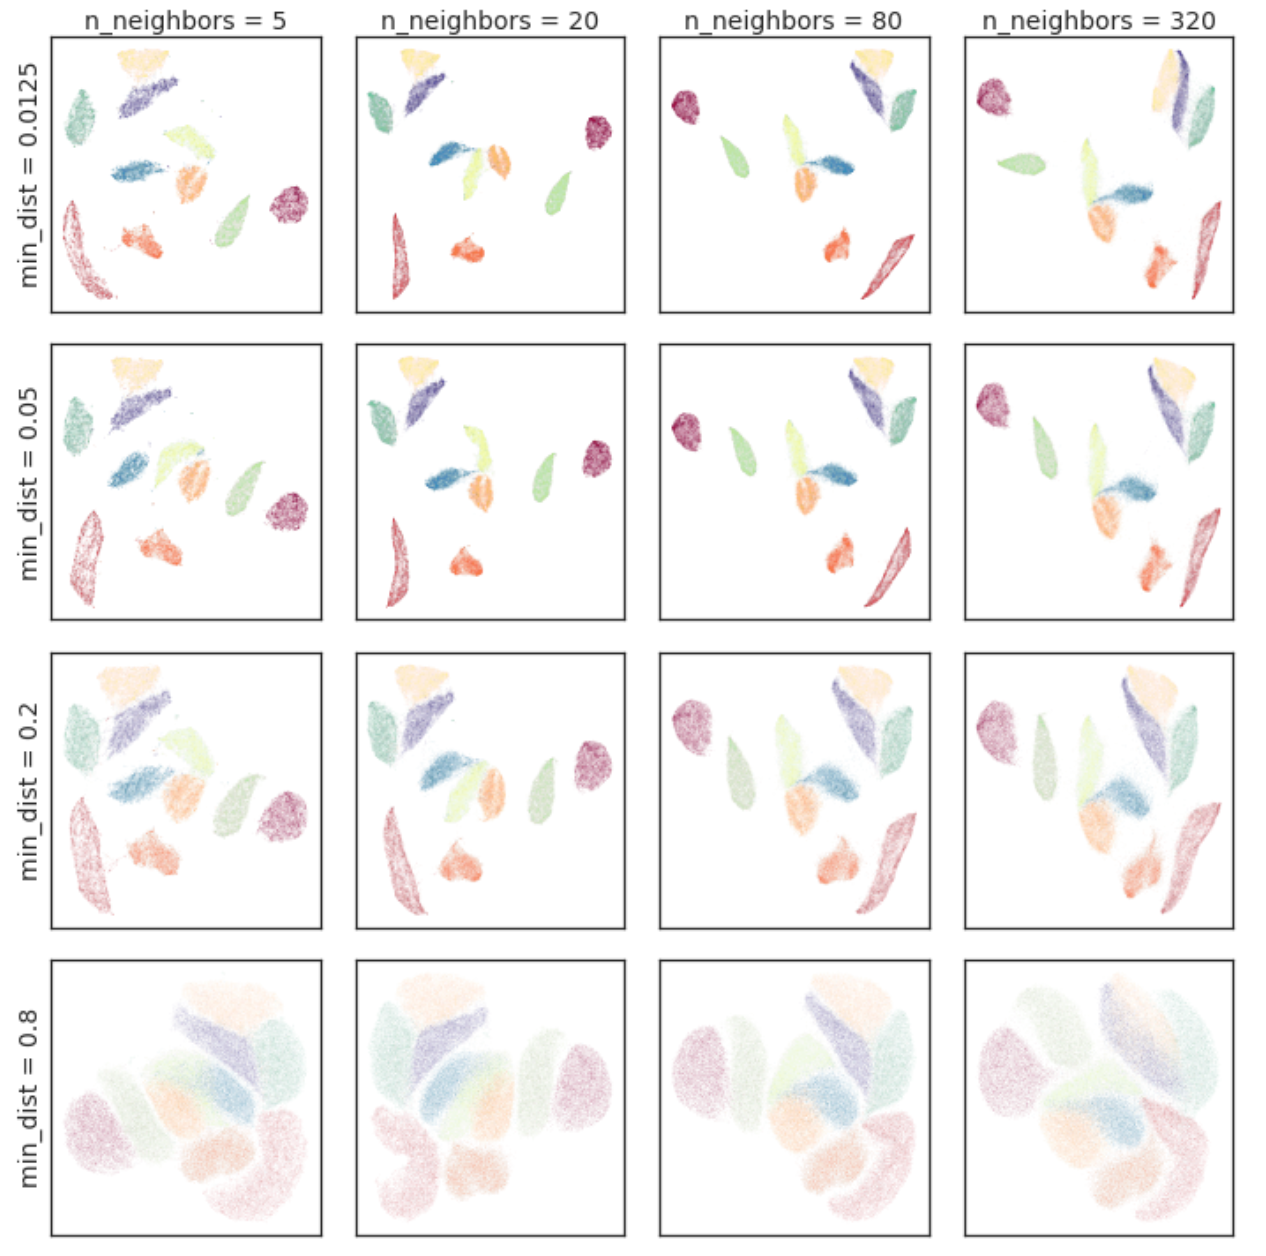
\includegraphics[width=0.9\textwidth]{img/umap_mnist.png}
    \end{minipage}
    \hfill
    \begin{minipage}{0.4\textwidth}
        \caption{Example of UMAP applied to the MNIST 10-digit dataset. The grid of scatter plots illustrates how varying the ``\(n_{\text{neighbors}}\)'' and ``\(\min_{\text{dist}}\)'' parameters affects the clustering behavior of the digits in the low-dimensional space.}
    \end{minipage}
\end{figure}

\subsection{Heat Kernel and Manifold Surface Distances}
When mapping a manifold surface into a network, we must distinguish between two fundamental types of distances:
\begin{itemize}
    \item \textbf{Geodetic distance between nodes:} This is defined topologically by the \textbf{shortest paths} walking along the edges of the graph.
    \item \textbf{Euclidean distance between nodes:} In the embedded space, this is the geometric distance between the \( K \) eigenvector components representing the nodes. As seen in the Young-Householder decomposition, this distance is weighted by the exponentiated eigenvalues (distance geometry).
\end{itemize}

\subsection{Applications: 2D/3D Delaunay Triangulation}
To apply spectral embedding to continuous objects (like images or 3D models), we must first discretize them into graphs.

\textbf{Delaunay triangulation} is a well-known algorithmic standard used to convert 2D planes or 3D surfaces into a strict nodes-and-edges representation (a mesh). Once the object is converted into a graph, we can apply spectral embedding techniques:
\begin{itemize}
    \item \textbf{Heat Kernel Evolution:} We can look for different object representations as a function of the kernel evolution time \( t \) (filtering details vs. macro-structures).
    \item \textbf{Laplacian Operator (Nodal Regions):} We can visualize the \( n \)-th eigenvector by mapping its component values back onto the physical object as colors. The sign changes (nodal points/regions) will naturally segment the object into structurally meaningful parts (e.g., separating the arms and legs from the torso of a 3D human model).
\end{itemize}

\begin{figure}[H]
    \centering
    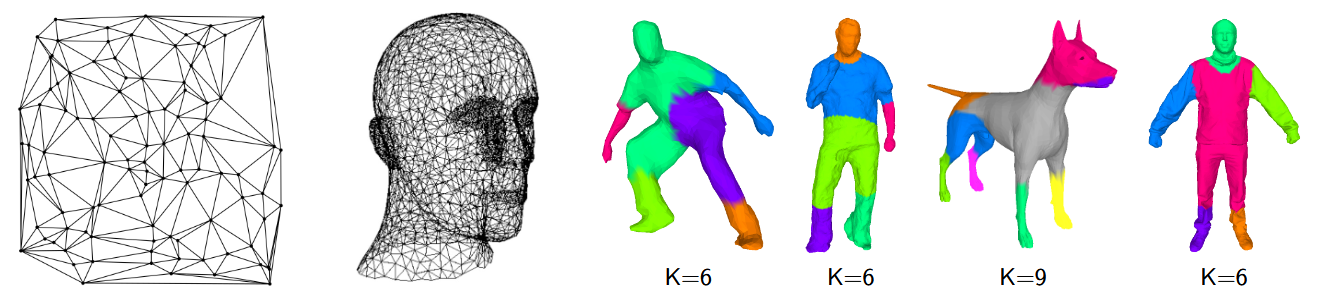
\includegraphics[width=0.8\textwidth]{img/heat_kernel_delaunay.png}
    \caption{Example of a 3D object (a human head, body and a dog) represented as a Delaunay triangulation mesh. The color coding represents the values of a specific eigenvector of the Laplacian, highlighting the nodal regions that segment the object into meaningful parts.}
\end{figure}

\subsection{Real-World Example: Italian Railway Network}
Node embedding can reveal whether a network's topology is dictated by geography or by functional logic. Consider the Italian Railway Network (\textit{Data source: viaggiatreno API}).

If we visualize the network using strict \textbf{geo-coordinates}, we clearly see the geographical shape of Italy. However, if we apply a \textbf{spring embedding} layout (using travel distance or time as weights, ignoring GPS coordinates), the topological shape distorts.
Plotting the \textbf{geographical distances vs. the spring layout distances} yields a scatter plot with a strong linear correlation, but with significant outliers. These outliers represent railway segments where topological proximity (e.g., a high-speed direct train) drastically "shrinks" the effective distance compared to what geography would suggest.

\begin{figure}[H]
    \centering
    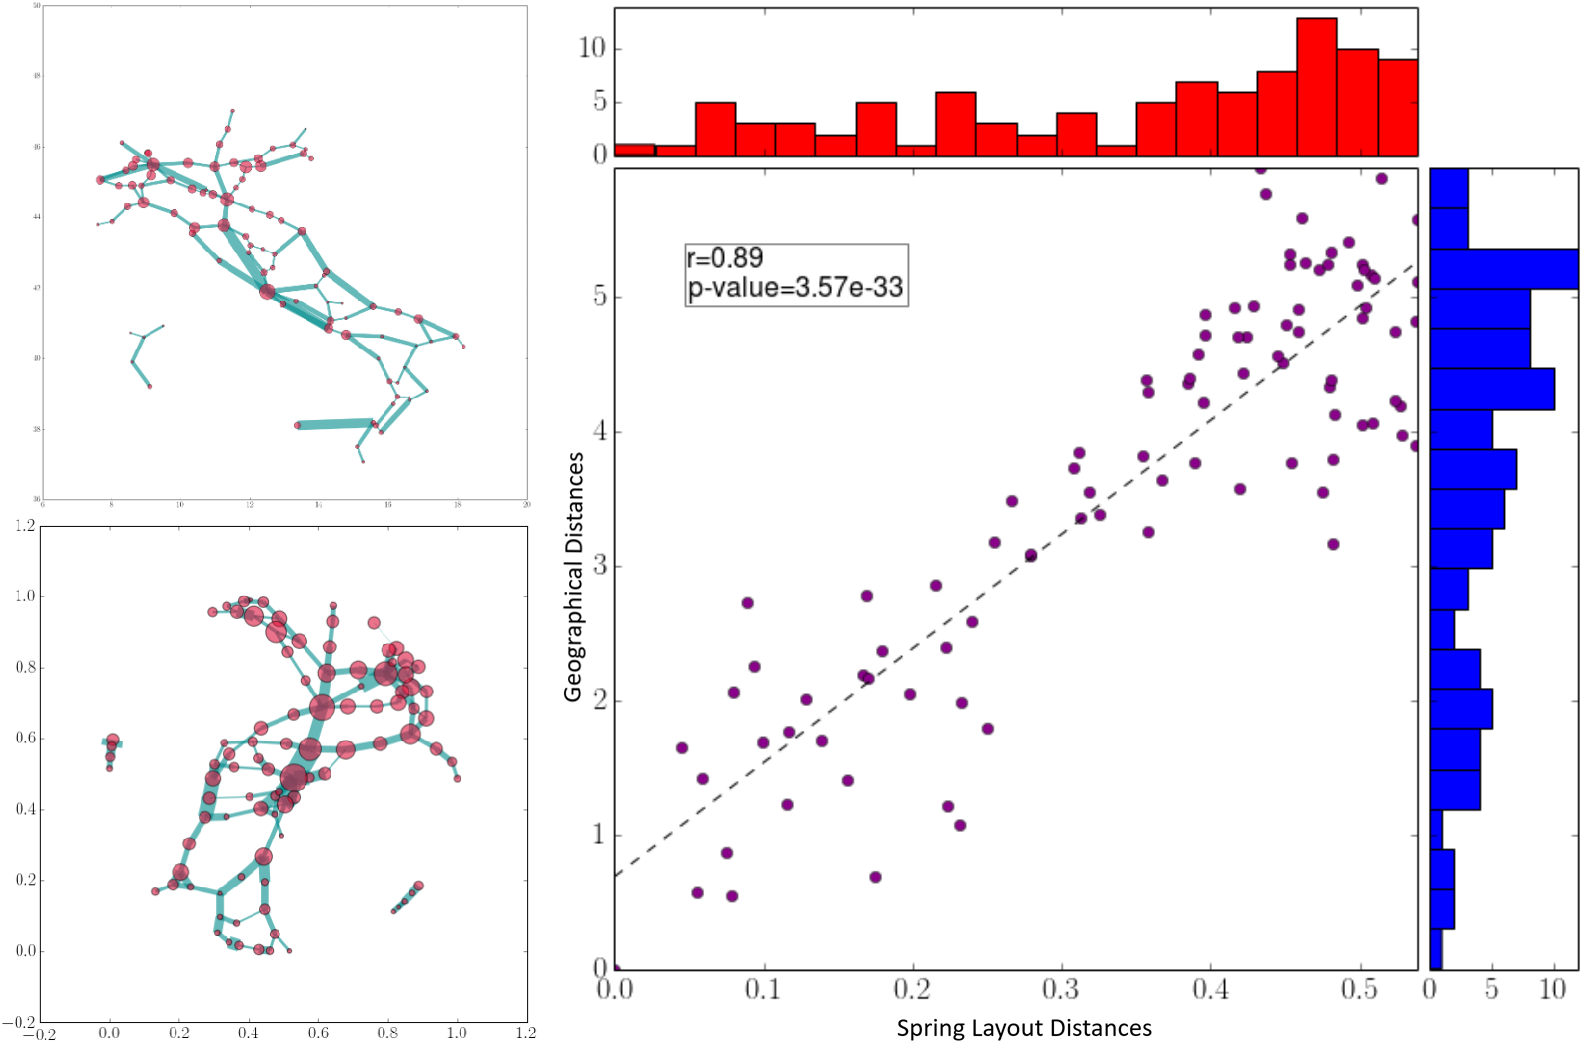
\includegraphics[width=0.8\textwidth]{img/italian_railway_network.png}
    \caption{Comparison of the geographical plot of the Italian railway network (top) with its topological spring embedding (bottom), alongside the scatter plot showing the correlation between geographical distances and spring layout distances.}
\end{figure}

\subsection{Standard Object Datasets for Network Analysis}
To test clustering, embedding, and manifold learning algorithms, researchers rely on standard benchmark datasets. Common datasets for transforming objects into graph networks include:
\begin{itemize}
    \item \textbf{MNIST:} A classic dataset of 70,000 grayscale handwritten digits, each \( 28 \times 28 \) pixels.
    \item \textbf{COIL20:} A dataset featuring 20 different grayscale objects photographed from different angles/orientations, at \( 128 \times 128 \) pixels.
    \item \textbf{ModelNet40:} The Princeton 3D Object Dataset (available for download on Kaggle), containing comprehensive 3D CAD models belonging to 40 different object categories, ideal for 3D mesh and spectral graph analysis.
\end{itemize}